\chapter{基于CAE-CNN的无线信号调制识别}

\section{引言}

无线通信领域的研究人员已经开始将深度神经网络应用于认知无线电,并取得了一定的成果\cite{migliori2016biologically}\cite{schmidt2017wireless}\cite{oshea2016convolutional}。
Oshea最近证明了利用原始数据进行有监督无线调制识别的可行性,
作者利用原始信号经希尔伯特变换后得到的$I$与$Q$路信号作为训练样本,调制方式作为标签,训练CNN分类器。
结果显示,其分类性能超越了传统的基于专家特征的决策树、SVM等分类模型。
然而,作者仅仅是用了传统的CNN框架,并没有对分类性能以及网络框架进行进一步的研究。\par

本章针对无线信号调制识别问题,提出了一种基于CAE与CNN融合的无线信号调制识别的算法框架,
并将此框架下的识别准确率及鲁棒性等与传统的基于特征的识别方法进行比较分析。\par

\section{调制信号}

无线通信信号实际上是经过调制信号与信道综合作用生成的。
尽管在机器学习中我们一般会建议使用真实数据,但是在无线电通信领域中,
由于标记数据匮乏,而且在现实中采集真实可靠的数据,是一种相当费时费力的工作,并且也很难得到监管部门的许可,
因此在我们的应用场景中,使用仿真数据进行实验较为普遍。
本文所用基础数据,经过纯粹的软件仿真,利用基础硬件进行信号生成与采集,相较于经过纯粹的软件仿真所得数据,
具备较高的可靠性。\par
\subsection{调制信号生成}
我们利用SMW200A信号生成器,构建通信系统框架,获取近似真实的仿真信号。
我们以与真实系统完全相同的方式确定性地引入调制,脉冲整形,携带数据以及与现实通信系统相同的发射参数。 
我们将真实的语音和文本数据集调制到信号上,这样,接收信号不仅是一系列的确知信号,并且包含了信息,
使我们的调制信号更接近真实环境中的信号。\par

信号源我们使用信号生成器生成随机信号,SMW200A信号生成器自带信道模型,这包括许多所需的信道,例如高斯信道,频率选择性信道、多径信道、瑞利信道等。
由于高斯信道统计特性较为确定,下文当中使用的数据,我们是利用高斯信道生成的数据。
但是,基于多径信道仿真的数据我们已经获取,后续将会利用更接近真实的数据继续进行相应的研究。\par

整个调制信号生成的系统框图如图\ref{sec:fig_3_1}所示。\par
\begin{figure}
	\centering
	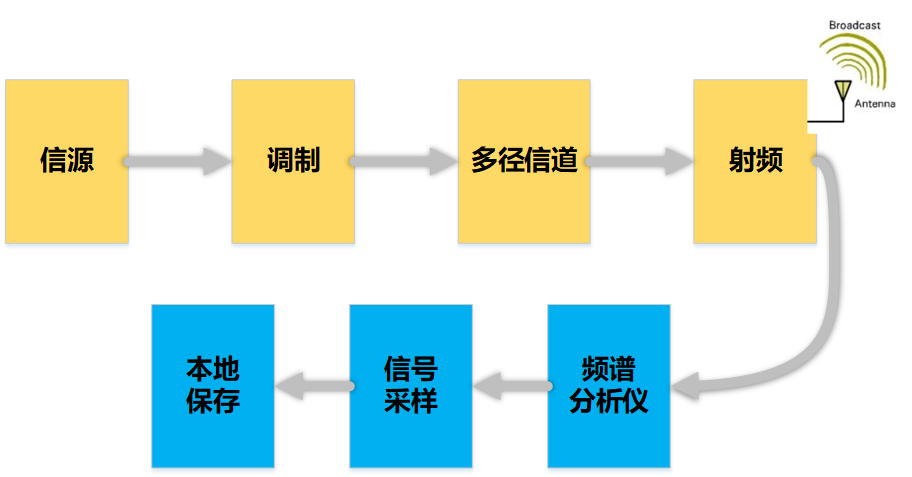
\includegraphics[scale=0.6]{./figures/chapter_3/fig_3_1}
	\caption{调制信号生成框图}\label{sec:fig_3_1}
\end{figure}
我们生成的数据集主要由7种调制方式组成:其中包括6类数字调制和1类模拟调制。这些调制方式都被广泛应用于我们周围的无线通信系统中,对于调制识别而言具备一定的代表性。
这些调制类别为AM-SSB, BPSK, CPFSK, GFSK, PAM4, QAM64, QPSK。

SMW200A信号发生器的需要调节的参数很多,在此我们列出了高斯信道条件下主要设置的部分系统参数,
如表\ref{tab:table_3_1}所示。\par
\begin{table}[!htbp]
	\centering
	\caption{SMW200A参数}\label{tab:table_3_1}
	\begin{tabular}{|c|c|c|}
		\hline
		\multirow{6}*{Baseband}
		& symbol Rate & 5M Sym/s\\ \cline{2-3}
		& Trigger In & Auto\\  \cline{2-3}
		& Clock & Internal\\ \cline{2-3}
		& Data Source & RRBS \\ \cline{2-3}
		& SNR & -20dB \textasciitilde 18dB\\ \cline{2-3}
		& Modulation &\tabincell{c}{
			AM-SSB, BPSK, CPFSK, GFSK,\\
			 PAM4, QAM64, QPSK		
		}\\ \cline{2-3}
		
		& Filter & \tabincell{c}{
			Gauss, Multi-Path, Rayleigh\\
			roll off factor=0.3}\\
		\hline
		
		\multirow{2}*{AWGN A}
		& System Bandwidth & 10MHz\\ \cline{2-3}
		& Mode & Additive Noise\\
		\hline
		
		\multirow{4}*{Others}
		& IQ Mod & open\\ \cline{2-3}
		& RF A & open\\ \cline{2-3}
		& Carrier & 1GHz\\ \cline{2-3}
		& Level &\tabincell{c}{
			(-20 \textasciitilde 10db) = -10dBm\\
			(-9 \textasciitilde 5db) = -5dBm\\
			(-4 \textasciitilde 18db) = 0dBm}\\
		\hline
	\end{tabular}
\end{table}

\subsection{信号采集}
在射频接收端,我们使用FSW50频谱分析仪接收经过多径信道后的样本,并查看其星座图和功率谱密度确定采样的准确性,最后将IQ两路采样数据保存到硬盘中。
并利用频谱分析仪对采样数据保存到本地,用于后续的调制识别研究。
FSW50频谱分析仪的系统参数如表\ref{tab:table_3_2}所示:\par

\begin{table}[!htbp]
	\centering
	\caption{SMW200A参数}\label{tab:table_3_2}
	\begin{tabular}{|c|c|c|}
		\hline
		\multirow{4}*{IQ Mod}
		& Sample Rate & 40 MHz \\ \cline{2-3}
		& Number of samples & 40000000\\ \cline{2-3}
		& Duration of signal & 1 s \\ \cline{2-3}
		& Data format complex & float32\\ \cline{2-3}
		& Scaling factor & 1 V\\ \cline{2-3}
		& Center frequency of I/Q capture & 1 GHz \\ \cline{2-3}
		& Modulation & Adaptive to Signal Source \\ \cline{2-3}
		& Data Format & .tar\\
		\hline
	\end{tabular}
\end{table}

我们的符号率为5M/s,采样率大约为40M/s,则每一个样本的持续时间约为25μs,每个样本大约包含125个符号,
它们含有经过信道带来的随机时间偏移,缩放,旋转,相位和噪声等影响。\par
数据以大约每个符号8次采样的速率进行采样,数据源的平均发送功率为0dB。\par
因此,我们使用1000个采样点的滑动窗口,在采样信号序列上滑动,每次移动1000个采样点,来获取训练样本。
最后我们将数据样本,以32位浮点数的复数形式保存成mat文件,总数据集大约30GB。\par


\section{调制信号的表示}

不同的调制信号具有不同的时频特征。本节,我们将原始数据可视化,了解不同信号的时频特征;
同时,我们利用CAE以及CNN获取信号的无监督表示,并展示不同信号在CAE特征空间中的分布状况,
从而进一步了解不同网络框架对调制信号进行特征提取的不同状况。

\subsection{数据集可视化}

对于每一种调制方式,我们随机抽出一个样本,并对其时域(图\ref{sec:fig_3_1})和频域(图\ref{sec:fig_3_2})进行展示。
我们可以发现,不同调制方式之间具备许多相似性,同时也具备一定差异性。有些信号我们是可以通过肉眼进行模糊判别;
但是,受脉冲形变,失真和其他信道影响,有些信号即便是人类专家也很难从视觉上分辨属于何种调制类别。\par

如图(图\ref{sec:fig_3_2})所示,在时域中,我们可以看到BPSK等信号具备较明显的特征,
而AM-SSB等信号在视觉上让人感觉像是噪声,很难直接判断出来。\par

\begin{figure}[!h]
	\centering
	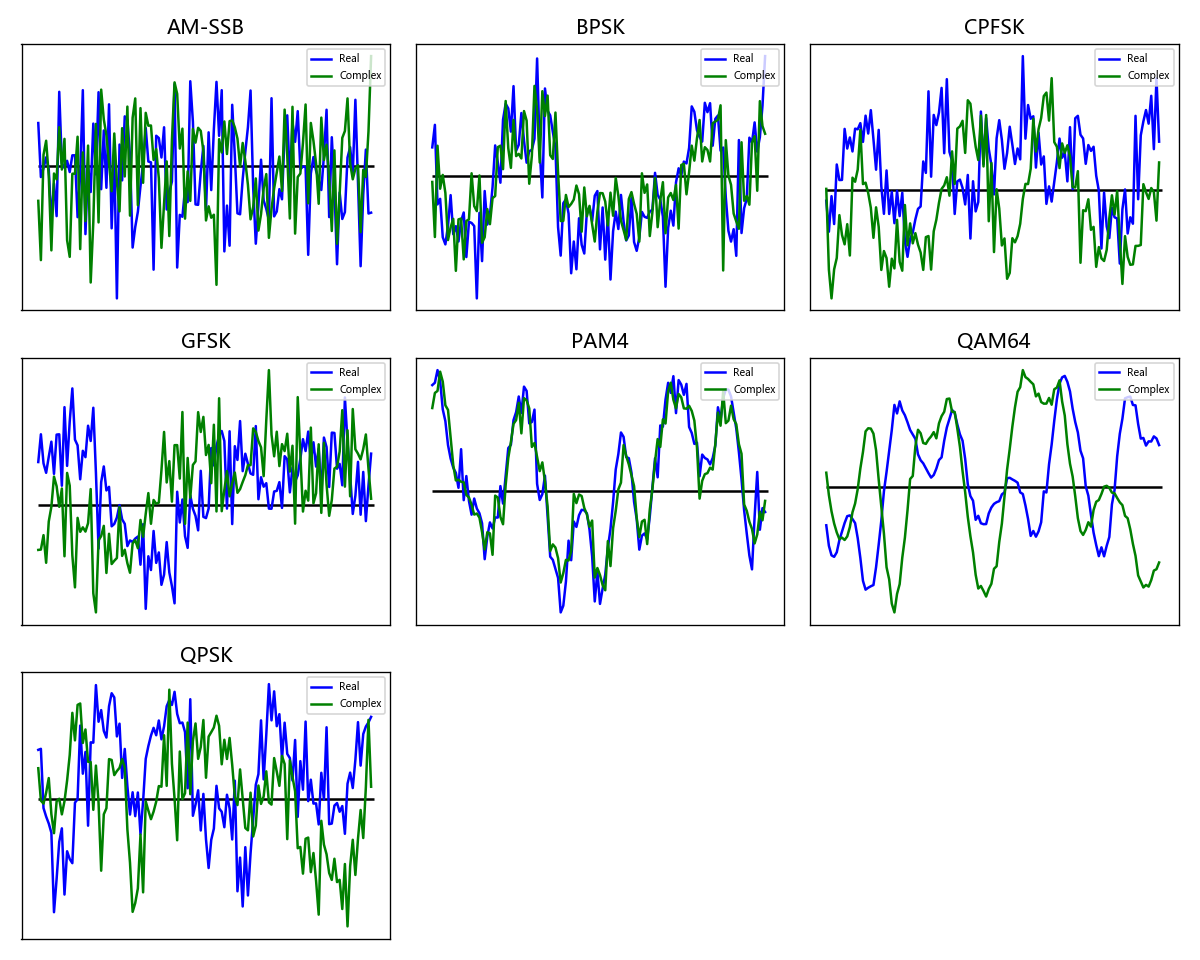
\includegraphics[scale=0.45]{figures/chapter_3/fig_3_2}
	\caption{不同调制方式的高SNR样本的时域波形}\label{sec:fig_3_2}
\end{figure}

如图\ref{sec:fig_3_3}所示,在频域中,每一个信号都具备一个带宽限制的功率包络,
其形状为调制识别提供了一定的信息,但是对于人类专家来说,从视觉来区分不同的调制信号是一个困难且繁琐的判定方法。\par
\begin{figure}[!h]
	\centering
	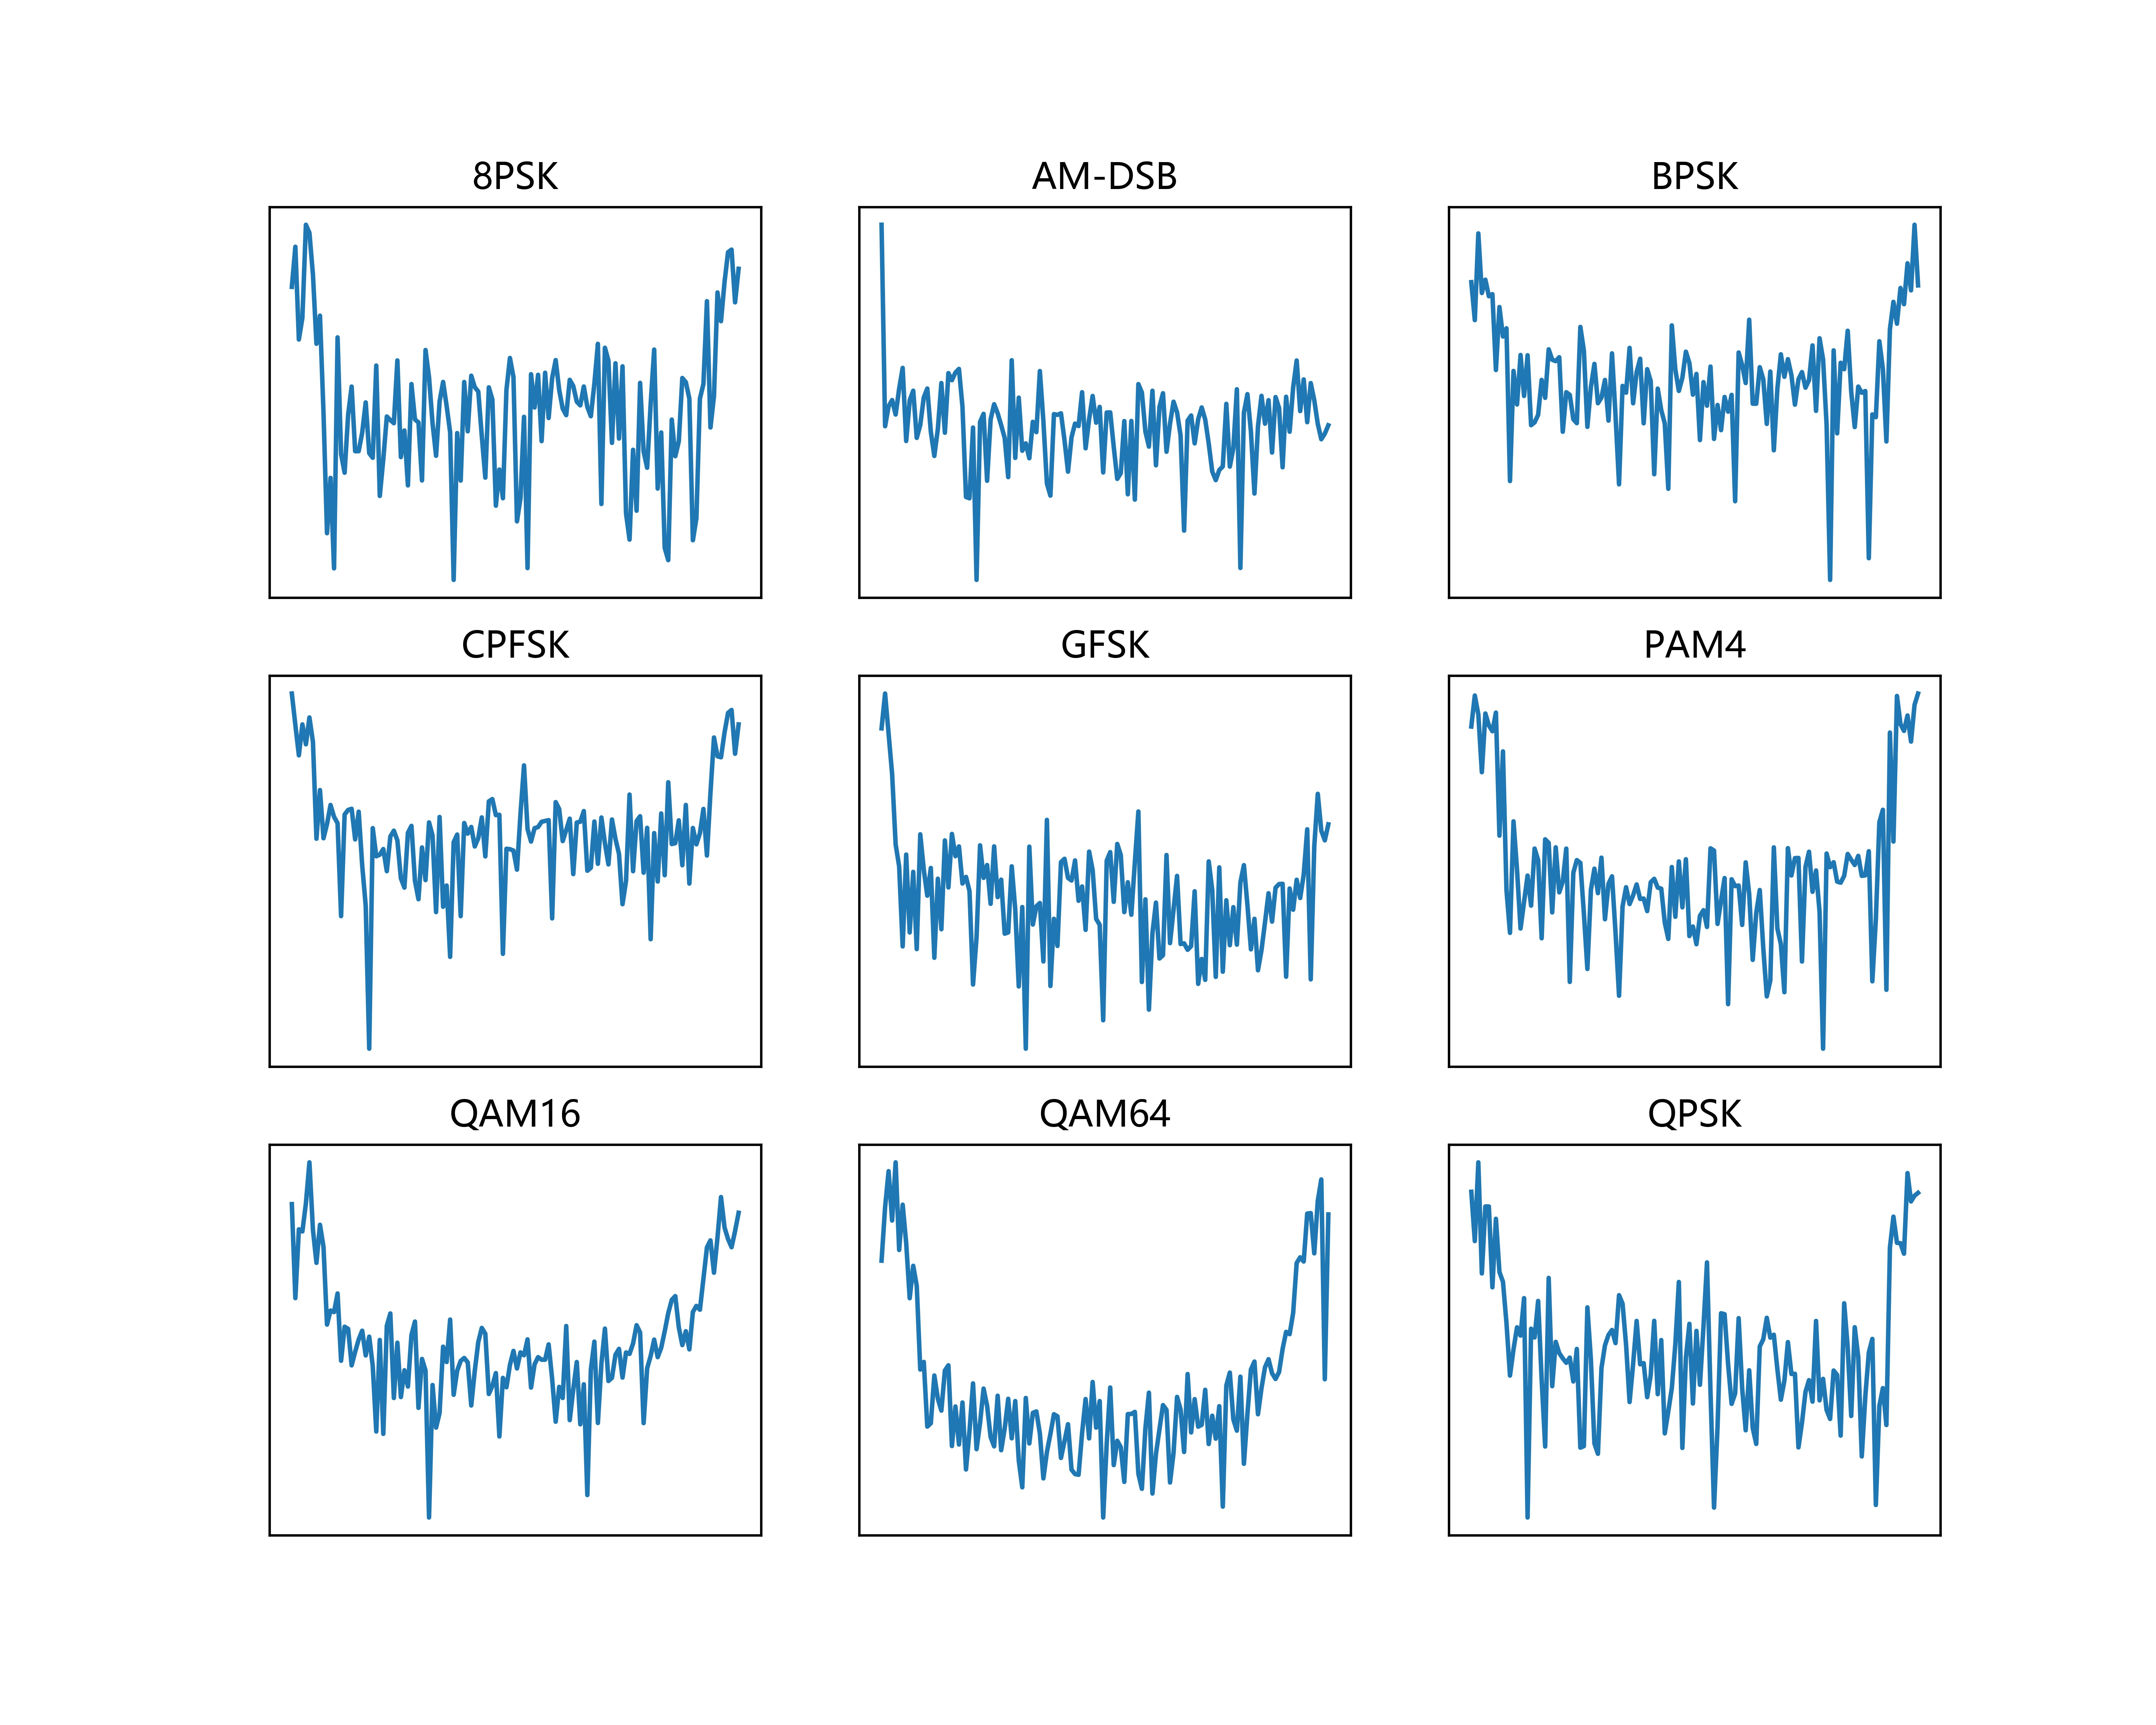
\includegraphics[scale=0.45]{figures/chapter_3/fig_3_3}
	\caption{不同调制方式的高SNR样本的频谱}\label{sec:fig_3_3}
\end{figure}

\subsection{调制信号的无监督表示}

无监督的稀疏表示是指在没有使用类标签的情况下,利用无监督的方法来学习数据集的稀疏表示。
这可以通过使用基于数据依赖性的降维技术来完成,例如主成分分析(Principal components analysis,PCA)
或独立分量分析(Independent components analysis,缩写:ICA)。
但是,这些方法只能对数据进行线性降维,如果说处于低维流型的数据与原始空间本身不具备线性关系,
那么这种情况下就不适合使用线性降维方法。\par

CAE非常适合于减小参数空间,获取的卷积特征具有时移不变性。
在CAE的训练过程中,我们尽量减少信号重构的MSE,但由于我们的主要目标是获得原始信号的聚类稀疏表示,
因此我们对重构误差作出简化假设:限制重构误差最小的情况下尽量降低隐藏层的维度。
然而,由于很难确定重构误差的最小值,
所以,我们只能人为的指定隐层的维度来确定我们的稀疏表示维度,在维度确定的情况下调整参数使重构误差尽量小。
本文中,我们利用卷积自编码器对输入的信号进行重构,学习一组原始信号的非线性稀疏表示。\par

自动编码器是一种无监督的学习算法,其中神经网络的优化目标是通过一些更有约束的中间维度,
使用MSE等损失函数,最小化输出处的重构误差。
通常,自编码器利用反向传播算法,将误差进行反向传播,并使用SGD算法等,
以找到接近等式\eqref{sec:eqt_3_1}中的最佳网络参数。

\begin{equation}\label{sec:eqt_3_1}
	\hat{\theta} = \mathop{\arg\min}_{\theta}(\sum(X − f (X,\theta))^2)
\end{equation}

通过约束网络的中间层维度,从而可以通过提取用于聚类的中间稀疏编码,来获得原始数据的非线性降维。
在这种情况下,使用相似的调制信号,可以由相似的卷积核和特征图来表示,因此,他们分布在该压缩空间的相近区域中。
自编码器中的卷积层具有时移不变性以及受约束的参数搜索空间(相对于全连接层),因此非常适合于无线电时间序列信号表示。
我们使用dropout等方法,并在输入层加入噪声对网络进行正则化,来增强模型的泛化能力。
图\ref{sec:fig_3_4}显示了卷积自动编码器的体系结构。

\begin{figure}[!h]
	\centering
	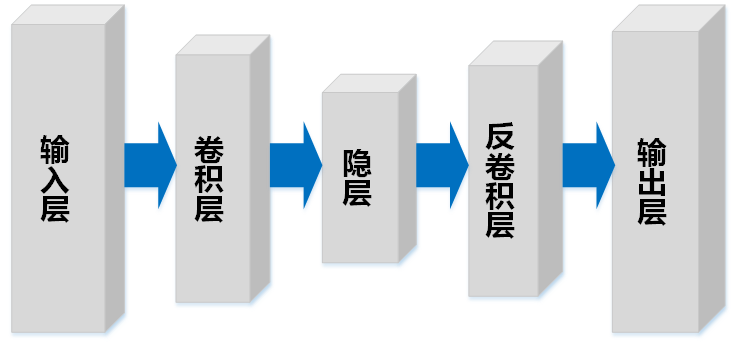
\includegraphics[scale=0.6]{figures/chapter_3/fig_3_4}
	\caption{自编码器}	\label{sec:fig_3_4}
\end{figure}

我们使用RMSProp和Adam梯度下降求解器进行优化,两者都获得了相似的结果,
下文中我们默认使用具备自适应学习速率的Adam优化器进行训练。\par

图\ref{sec:fig_3_5}显示了两个输入维度为$2 \times 128$的训练样本,中间隐层维度为$1 \times 30$,
以及输出维度为$2 \times 128$的训练结果展示图。\par
\begin{figure}[!h]
	\centering
	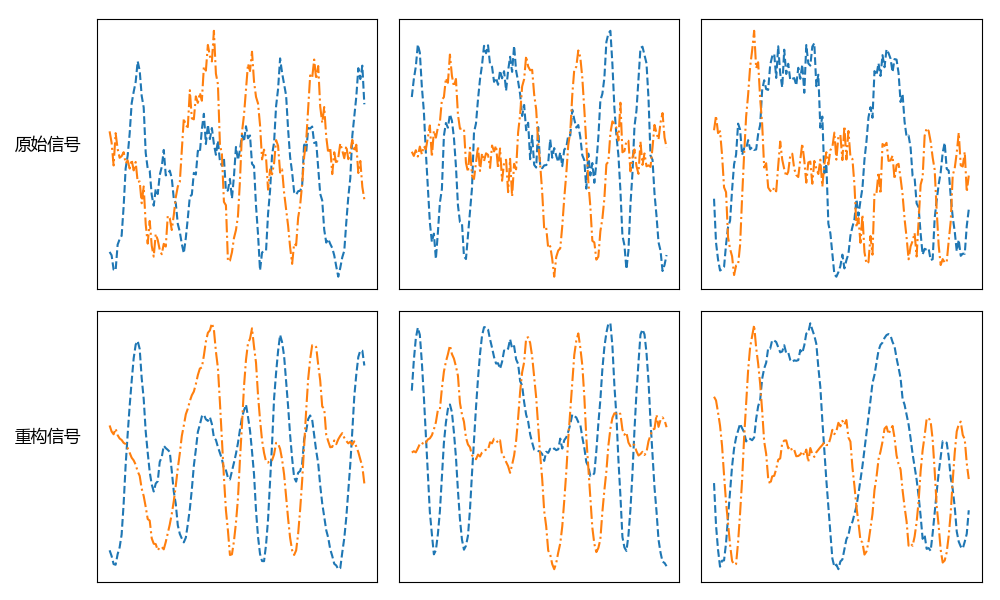
\includegraphics[scale=0.6]{figures/chapter_3/fig_3_5}
	\caption{基于自编码器的信号复现}	\label{sec:fig_3_5}
\end{figure} 

通过图\ref{sec:fig_3_5},我们可以发现,卷积自编码器可以很好的复现原始信号;
我们提取的特征可以很好地重构原始数据,即可以很好地表征原始数据。
这说明我们的卷积自编码器可以通过无监督的方式学习信号的低维嵌入表示。\par

为了可视化我们学到的卷及特征,并对这些特征的类可分性进行直观展示,我们将数据的低维嵌入特征,
利用t-SNE算法映射到二维流型,并在平面坐标系中展示。
在低维嵌入空间中分布在相近的区域的样本,分布在二维流型中相近的区域。
因此,我们可以通过观察不同类别的数据样本在t-SNE可视化之后的二维流型上的分布,来反映样本无监督表示的类可分性。\par

我们训练卷积自编码器从每一类样本中随机采样100个样本,将其通过训练的卷积自编码器获得其低维无监督表示,
并利用t-SNE映射到二维流型,最终的效果如图\ref{sec:fig_3_6}。

\begin{figure}[!h]
	\centering
	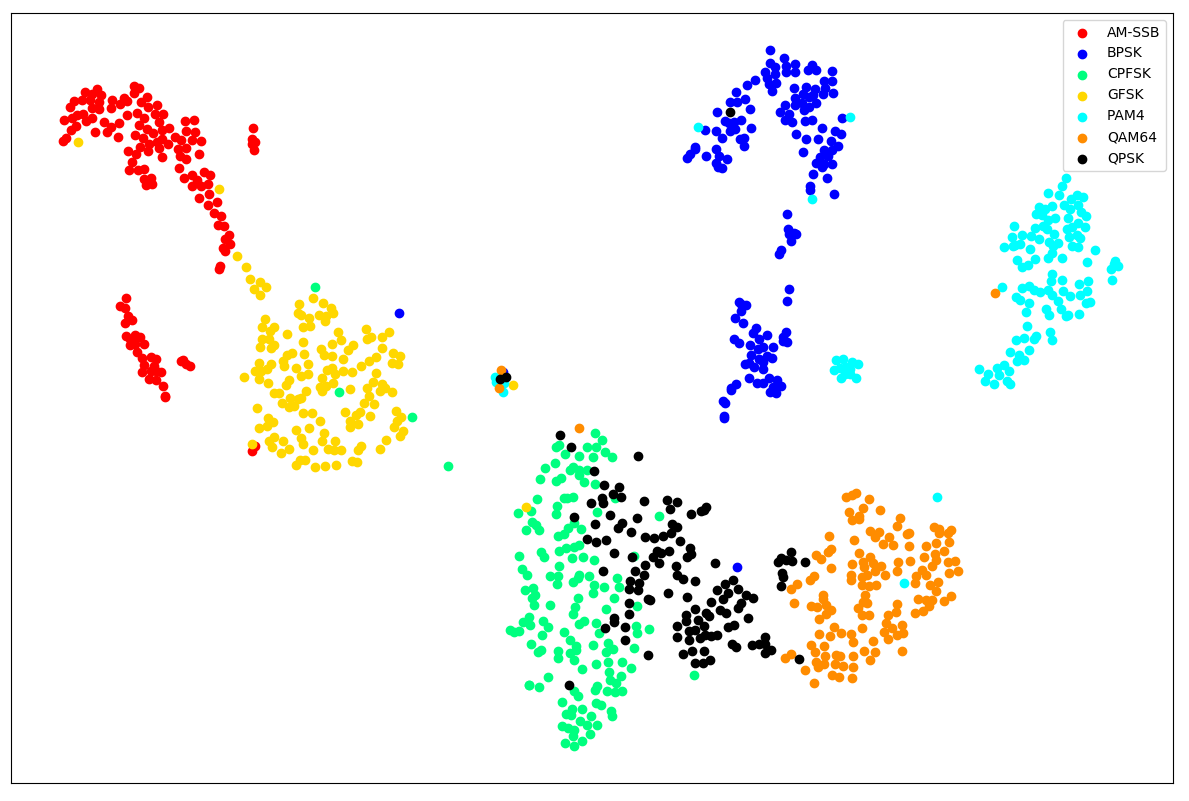
\includegraphics[scale=0.4]{figures/chapter_3/fig_3_6}
	\caption{基于自编码器的调制信号t-SNE二维流型展示}	\label{sec:fig_3_6}
\end{figure}

在这种情况下,我们看到几个类如QAM64,AM-SSB,PAM4和BPSK已经形成了独立的、大部分可分的簇,
可以利用DBSCAN等聚类方法聚类为单独的类;而其他类则会出现类别混淆,并且难以通过聚类方法分离类别簇。 
尽管我们的无监督表示类可分性效果不太好,但考虑到这些特征从来没有被训练用来区分不同类别的样本,
我们就已经获得了数据一定程度的类可分性,这已经算是一个可以接受的结果了。 \par 

\subsection{调制信号的监督引导稀疏表示}

当我们具有一部分监督数据的时候,我们也可以使用监督训练时学习到的判别特征生成一个稀疏表示空间。
OShea在他的工作中,利用有标记样本以监督方式训练卷积神经网络,可以达到很好的分类效果。
CNN主要是由卷基层与DNN层构成;由于CNN本身可以对测试样本进行分类,这就相当于在进行Softmax层的分类之前,
我们已经获取了原始数据具有类别区分度的特征。
因此,我们可以利用监督的方式,获取原始数据的监督引导特征。\par

在训练好分类网络以后,我们移除最后的softmax层,保留剩余的这一部分网络。
这样,在样本经过训练好的网络,最后隐层输出的特征即为原始数据的稀疏表示。
我们利用监督方式训练网络,并获取监督引导特征空间,获取数据监督引导的稀疏表示。\par
我们从每一类样本中随机采样100个样本,通过图X的网络将其映射到监督引导特征空间,并利用t-SNE映射到二维流型,最终的效果如图X:
\begin{figure}[!h]
	\centering
	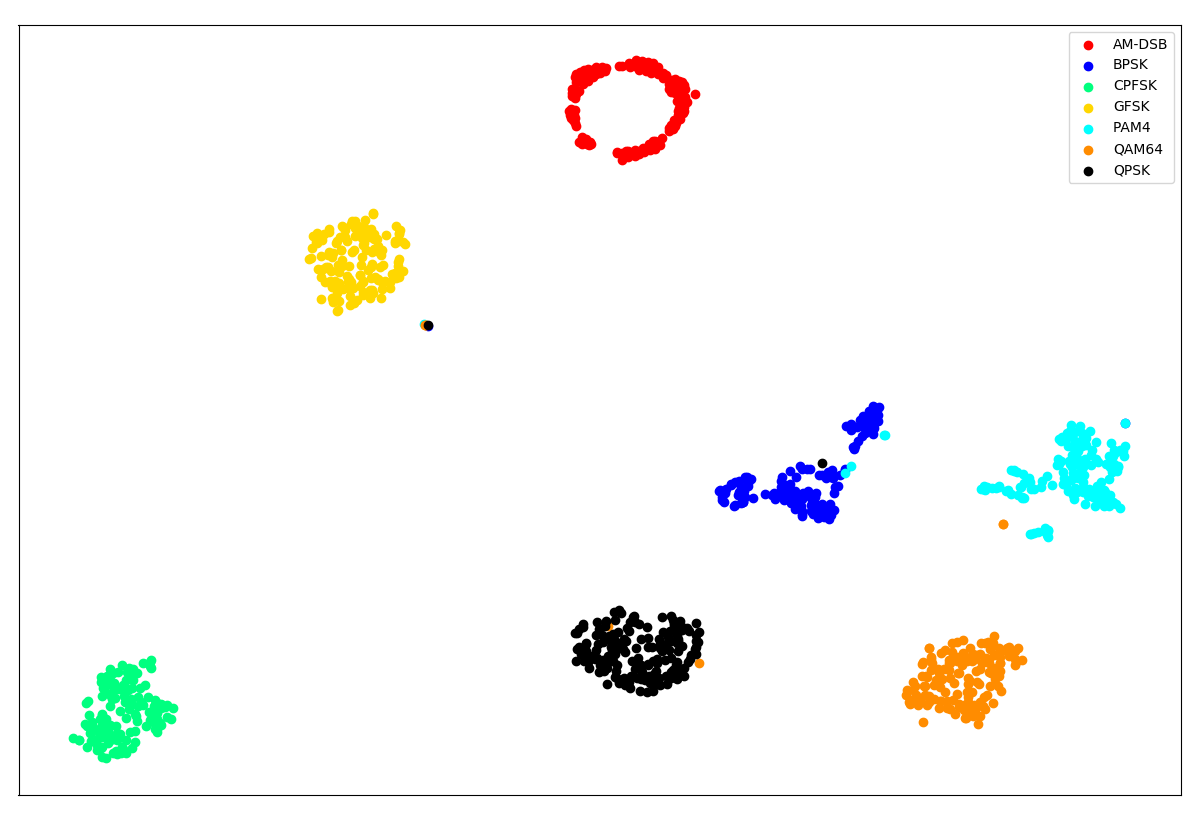
\includegraphics[scale=0.4]{figures/chapter_3/fig_3_7}
	\caption{基于CNN的调制信号t-SNE二维流型展示码器}	\label{sec:fig_3_7}
\end{figure}

在这种情况下,我们几乎可以把每个调制类别的样本在二维流型中利用聚类算法分开。
当然,其中也有一部分的数据是混淆的,比如类别X中也有部分样本散落到类别X中。\par
可能是因为在获取监督引导特征空间时,我们的目标是正确区分不同的调制类别,
所以我们获取的监督引导特征对于不同类别的样本是有一定的区分度的,即不同调制类别的样本分布在特征空间的不同区域,
这就表现为在t-SNE之后不同类别样本分布在二维流型的不同区域。
当然,随着训练网络时样本类别的增加,我们获取的具有类区分度的特征将会得到更好的泛化。\par


\section{基于CAE-CNN的无线信号调制识别}

在上一节中,我们分别使用监督引导和无监督引导的方法获取数据的低维表示,其本质上就是基于降维的非线性特征提取过程。
在本节中,通过融合CAE与CNN,我们联合重构误差与分类误差,提出了一种新的调制识别网络框架和训练算法。

\subsection{CAE-CNN网络框架}
在上一节中,我们发现数据样本在低维嵌入空间中的表示具有一定的类可分性。因此,我们可以将CNN分为特征提取与分类两个步骤。
对于CAE与CNN的融合,我们的本质是希望能够在分类的同时保证特征提取尽量多地包含数据的原始信息。
为此,我们通过在CNN的交叉熵损失中加入CAE的重构误差损失作为我们的整体损失;
通过改进CAE与CNN的训练算法,降低重构误差与分类误差,达到更好的分类效果。
图\ref{sec:fig_3_8}展示了我们网络的结构。

\begin{figure}[!h]
	\centering
	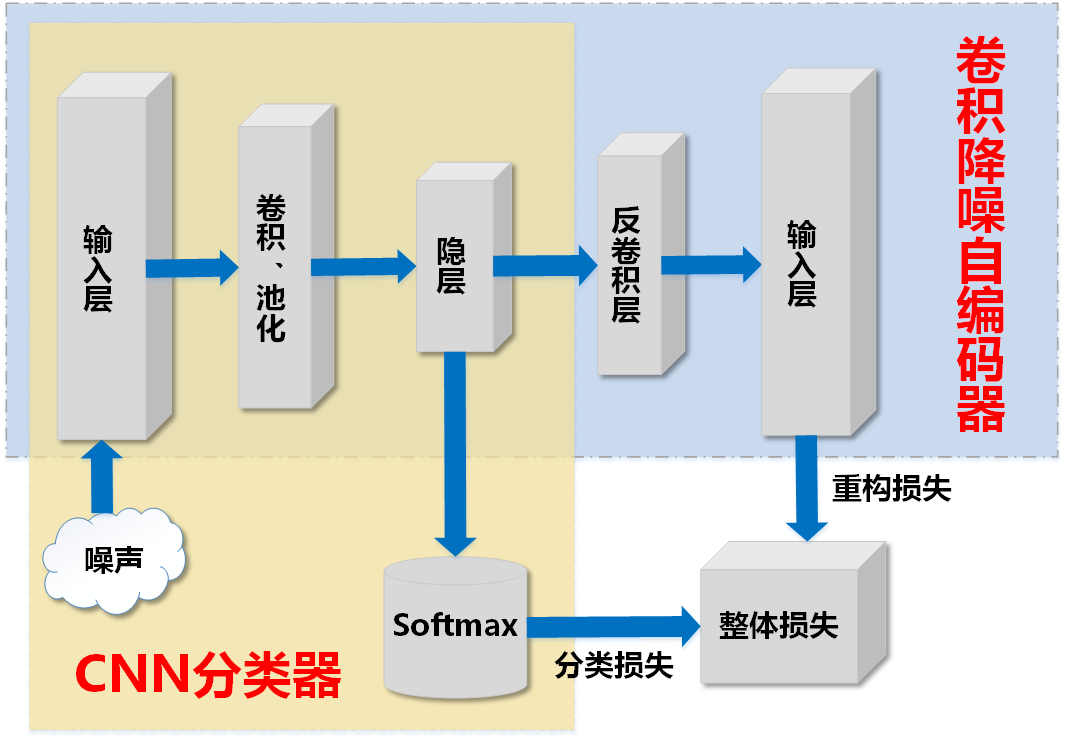
\includegraphics[scale=0.5]{figures/chapter_3/fig_3_8}
	\caption{CAE-CNN网络框架}	\label{sec:fig_3_8}
\end{figure}

在CAE-CNN中的卷基层中,我们使用了Dropout,用以降低模型的过拟合影响;
并在卷积权重增加了权重值$W$的2范数$||w||_2^2$作为惩罚项,使权重尽量小;
同时,借鉴稀疏自编码器(Sparse Autoencoder, SAE)的思想,
我们在第一个密集连接层加入权重的$F1$范数范数惩罚来鼓励解的稀疏性\cite{le2013building}。\par

那么我们有CAE的损失函数:
\begin{equation}\label{sec:eqt3_3}
	J_{CAE}(X, \hat{X}; \theta_{CAE}) = 
	\frac{1}{m}\sum_{i=1}^{m}||x^{(i)} - \hat{x^{(i)}}||_2^2  
	+ \frac{\lambda}{2}||w||_2^2 
	+ \eta||J_f(x)||_F^2
\end{equation}
其中,$J_f(x)$是隐层输出值对于权重的雅克比矩阵,$||J_f(x)||_F^2$表示该雅克比s矩阵$F$范数的平方。\par

由于CNN的损失函数我们使用交叉熵损失函数,同时将卷基层权值的二范数作为损失的一部分,那么我们有CNN的损失函数:
\begin{equation}\label{sec:eqt3_4}
	J_{CNN}(X, Y; \theta_{CNN}) = 
	\left[ \frac{1}{m} \sum_{i=1}^m \left( \frac{1}{2} \left\| h_{W,b}(x^{(i)}) - y^{(i)} \right\|^2 \right) \right]
	+ \frac{\sigma}{2} ||w||_2^2
\end{equation}

系统的总体损失函数为CAE的损失跟CNN损失的加权和,如方程\eqref{sec:eqt3_5}:
\begin{equation}\label{sec:eqt3_5}
	J(X, \hat{X}, Y; \theta_{CNN}, \theta_{CAE}) = 
		\alpha J_{CNN}(X, Y; \theta_{CNN}) 
		+ \beta J_{CAE}(X, \hat{X}; \theta_{CAE})
\end{equation}

\subsection{CAE-CNN算法}
在提出的CAE-CNN框架中,我们有分类损失与重构损失,因此在模型训练时,需要我们同时考虑到两种损失,
并进行反向传播得到优化后的网络参数。对应于我们的CAE-CNN框架,我们提出了\ref{alg:CAE_CNN}训练算法。

\begin{algorithm}[ht]
	\caption{CAE-CNN训练算法}
	\hspace*{0.02in} {\bf Input:}
	$\alpha, \beta, \lambda, \delta, \eta, K$
	
	\hspace*{0.02in} {\bf Output:}
	$J(X, \hat{X}, Y; \theta_{CNN}, \theta_{CAE}), 
	J_{CNN}(X, Y; \theta_{CNN}) ,
	J_{CAE}(X, \hat{X}; \theta_{CAE})$
	
	\label{alg:CAE_CNN}

	\begin{algorithmic}[1]
		\REQUIRE 初始化$\alpha, \beta, \lambda, \delta, \eta$
		\REQUIRE 初始化$K=1000, \Delta K=20, k=0, \Delta J=0.001, \Delta S=1000$
		\REQUIRE 训练数据集及测试数据集构建
		\REQUIRE 构建CAE框架及损失函数$J_{CNN}(X, Y; \theta_{CNN})$, 
		CAE框架及损失函数$J_{CAE}(X, \hat{X}; \theta_{CAE})$,
		以及整体损失函数$J(X, \hat{X}, Y; \theta_{CNN}, \theta_{CAE})$,
		最终构建完整的计算图Graph
		
		\WHILE{K>0}
			\FOR {$k=0; k<K; k=k+\Delta K$}
				\STATE 计算$J_{CAE}(X, \hat{X}; \theta_{CAE})$,并训练CAE网络
			\ENDFOR
			
			\FOR{$k=0; k<1000-K; k=k+\delta K$}
				\STATE 计算$J_{CNN}(X, Y; \theta_{CNN})$,并训练CNN网络
			\ENDFOR
			\STATE $K = K - 20$
		\ENDWHILE
		
		\STATE $S^* = 0$,$J_{CNN}^*=1e5$ 
		\FOR{$S = 1; \Delta S \leq  5000 || S>10^5; S++$ }
			\STATE 计算$J_{CNN}$,并训练$CNN$
			\IF{$J_{CNN} < J_{CNN}^*$}
				\STATE $J_{CNN}^* = J_{CNN}$
				
				\STATE $S^* = S$
			\ELSE
				\STATE $\Delta S = S - S^* $
			\ENDIF
			
			\IF{$S\%10 == 0$}
				 \STATE 计算$J_{CAE}$,并训练$CAE$
			\ENDIF
		\ENDFOR
	\end{algorithmic}
\end{algorithm}


\subsection{算法运行环境及参数}
使用分类交叉熵损失函数和Adam[15]求解器进行训练(在我们的数据集上略胜过RMSProp[12])。
我们在tensorflow[16]计算框架上运行网络的训练和预测,使用NVIDIA Cuda[8]组件,
在Nvidia GTX1080ti显卡上加速运算。接下来的仿真我们都使用这一套软硬件组合进行仿真。
我们的机器系统配置如表\ref{sec:table_3_1}所示。\par

%\begin{table}[H]
%	\centering
%	\caption{系统参数配置}
%	\begin{tabular}{|c|c|c|}
%		\hline
%		参数 & 配置\\ \hline
%		System & Ubuntu 17.10\\ \hline
%		CPU & Intel\textsuperscript{\textregistered}  Xeon(R) CPU E5-2683 v3 \\ \hline
%		GPU & GeForce GTX 1080 Ti\\ \hline
%		Memory & 64GB\\ \hline
%		HardDisk & 1TB\\ \hline
%		Python & python3.6\\ \hline
%		Library & Tensorflow1.4\\ \hline
%	\end{tabular}
%	\label{sec:table_3_1}  
%\end{table}

\begin{table}[H]
	\centering
	\caption{系统参数配置}
	\begin{tabular}{ccc}
		\toprule
		参数 & 配置\\
		\midrule
		System & Centos7.3\\
		\midrule
		CPU & Intel\textsuperscript{\textregistered}  Xeon(R) CPU E5-2683 v3 \\
		\midrule
		GPU & GeForce GTX 1080 Ti $\times$ 2\\
		\midrule 
		Memory & 32GB\\
		\midrule 
		Storage & 128G SSD \& 2TB HardDisk\\
		\midrule
		External Storage & Toshiba HDTH310E 2TB\\
		\midrule 
		Python & python3.6\\
		\midrule 
		Library & Tensorflow1.4\\
		\bottomrule
	\end{tabular}
	\label{sec:table_3_1}  
\end{table}

\section{结果及分析}
我们使用Adam优化器,CAE-CNN模型训练了大约需要50分钟。我们设置$BatchSize$大小为1024的样本,每一次训练集大约需要15秒。在epoch大于200之后,我们确实观察到一些过度拟合,因此在算法\ref{alg:CAE_CNN}中我们设置最大的循环次数小于300次epoch。\par

\subsection{分类结果}
我们调制方式总共有7种,每一类调制信号在噪声信噪比为$-20dB \sim 18dB$之间每隔$2dB$进行数据采样,
每个信噪比下采样0.1秒,每个样本共包含1000个采样值,大约有4000个样本。
我们将80\%的样本作为训练集,10\%的样本作为验证集集,10\%的样本作为测试集。
即训练样本大约有。 这些样本均匀分布在从-20dB到+18dB的SNR中,并被标记以便我们可以评估特定子集上的性能。\par

经过CAE-CNN的网络训练,我们在测试数据集上的所有信噪比之间的分类准确率大致达到了72.3%。这表示的是我们分类器在-20dB到18dB之间样本的一个平均准确率,由于信噪比在-2dB到-6dB之间分类器性能迅速下降至30\%左右,并在较低信噪比条件下维持一个很低的分类水平。因此,从这方面而言,这个准确率已经很高了。
最终, 我们CAE-CNN分类结果如图\ref{sec:fig_3_9}\par

\begin{figure}[!h]
	\centering
	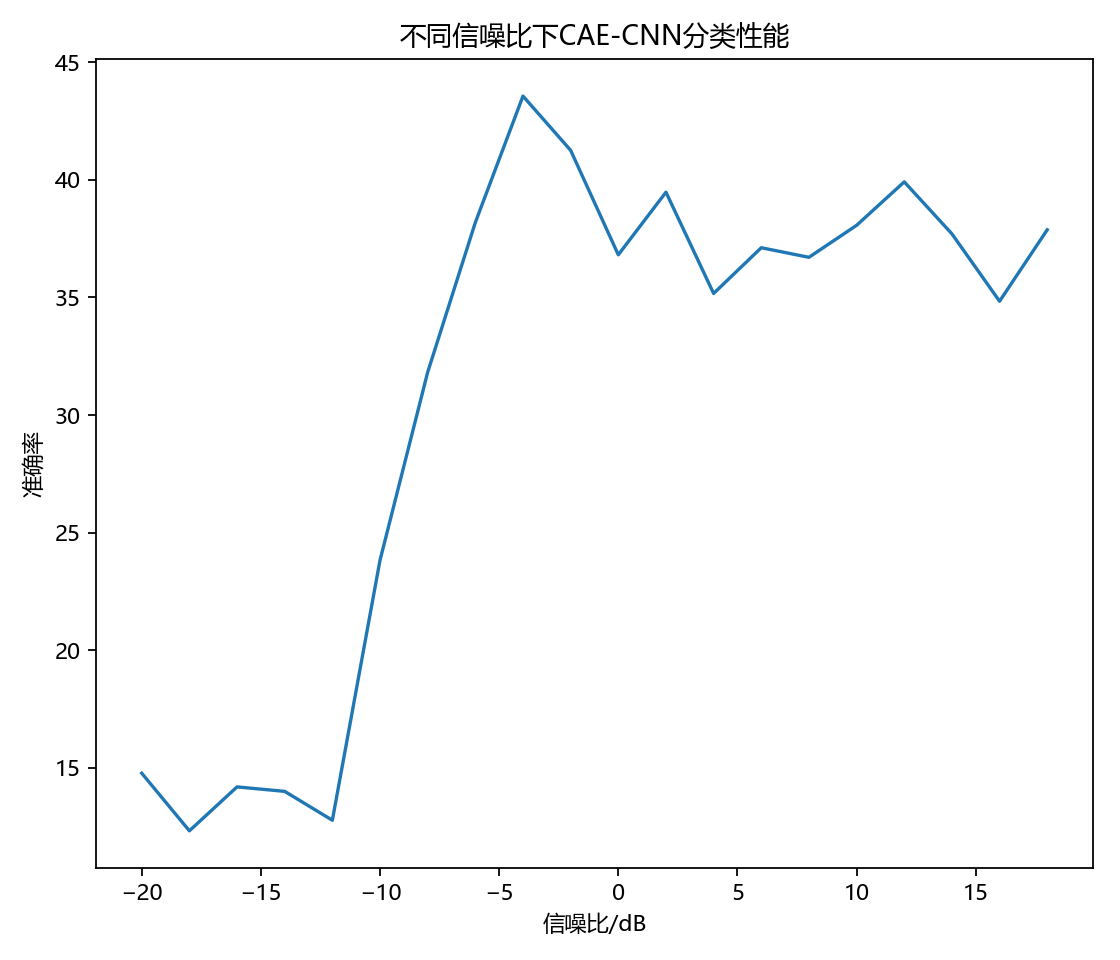
\includegraphics[scale=0.7]{figures/chapter_3/fig_3_9}
	\caption{CAE-CNN分类结果}	\label{sec:fig_3_9}
\end{figure}

从图\ref{sec:fig_3_9}中我们可以看出,信噪比在0dB以上时分类准确率都能达到96\%以上。在-4dB时,仍然有85\%以上的准确率,这相对于传统的基于特征的分类器而言,具有很大的提升。\par

同时,我们与前人提出的一些算法进行比较,
本文中我们选用了基于特征的支持向量机(Support Vector Machine,SVM)、决策树(Decision Tree,DTree)、
随机森林(RandomForest, RF)、K-近邻(K-NearestNeighbor,KNN)、
深度神经网络(Deep Neural Network, DNN)。分类器所用特征在第四章我们将系统阐述。最终,分类结果如图\ref{sec:fig_3_11}所示。\par

\begin{figure}[!h]
	\centering
	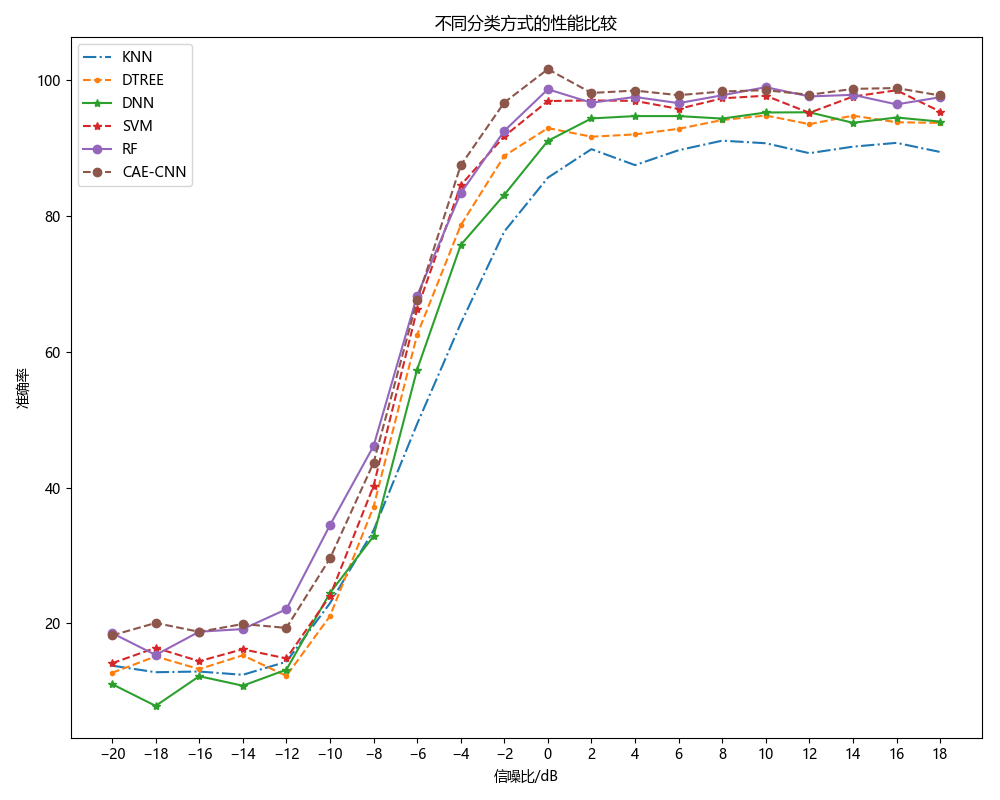
\includegraphics[scale=0.5]{figures/chapter_3/fig_3_11}
	\caption{与其他方法的比较}	\label{sec:fig_3_11}
\end{figure}

从图\ref{sec:fig_3_11}中我们可以看出,KNN大部分情况下分类性能较差;
在高信噪比(大于0dB)条件下,SVM、CAE-CNN和RF分类性能相差不大,
但是CAE-CNN性能相对更好一些,而且曲线比较平滑,分类性能较为稳定;
而在低信噪比条件下,CAE-CNN同时也具备较好的表现,大部分情况下优于其他的分类器。
由此可见,本文提出的调制识别算法具有较好的识别性能。\par

我们计算得到0dB的测试样本的分类混淆矩阵,并将其可视化,如图\ref{sec:fig_3_10}。\par
\begin{figure}[!h]
	\centering
	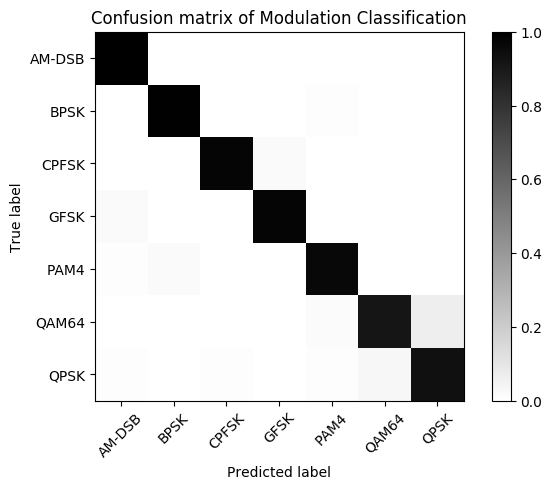
\includegraphics[scale=0.7]{figures/chapter_3/fig_3_10}
	\caption{0dB条件下的结果}	\label{sec:fig_3_10}
\end{figure}
可以看到SNR为0dB时,在混淆矩阵中我们有一个较为纯净的对角线,仅仅有少量的QPSK样本误分为BPSK和CPFSK。这可能与QPSK本身的相位和幅值同时变化有关,加之噪声带来一定的影响,使得分类器产生了个体样本的误判。\par

\subsection{算法效率}

由于调制识别的应用场景大都要求我们需要能够对信号进行实时响应,因此算法的运行效率将会是影响识别性能的重要因素。
在本节中,我们将通过比较不同算法的训练时间以及分类时间,查看算法的运行效率。由于不同算法的训练时间和样本分类时间在数量级上可能不同,所以接下来进行时间分析时,我们的时间坐标轴都是以对数坐标为基准的。\par

影响算法训练时间因素很多,包括能够实现并行、是否进行加速、算法复杂度、硬件设备、数据样本数目等等。
本文中所有测试算法均在同一平台下运行。
深度学习的一个普遍缺点是需要很大的计算量,然而在本文中,我们的网络相对较小,数据集的量也较少,在DNN和CAE-CNN的训练使用Tensorlow框架,并启用了GPU并行加速;KNN、SVM、RF、DTREE我们使用scikit-learn库中的API。最终的训练时间如图\ref{sec:fig_3_12}。\par
\begin{figure}[!h]
	\centering
	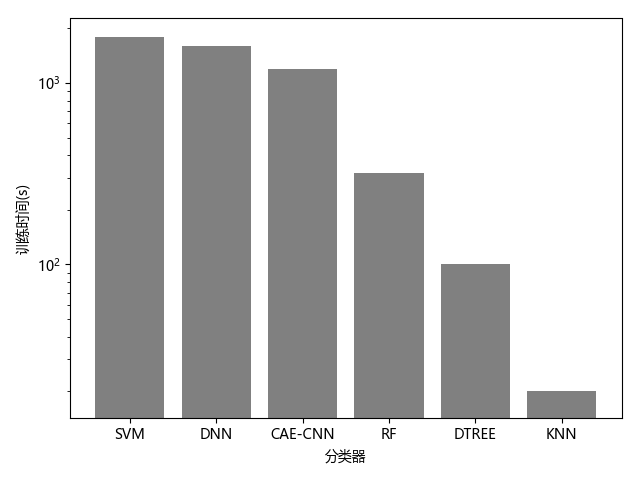
\includegraphics[scale=0.65]{figures/chapter_3/fig_3_12}
	\caption{不同算法训练时间}	\label{sec:fig_3_12}
\end{figure}
从图\ref{sec:fig_3_12}中我们可以看到,
KNN的训练时最快的,这是因为算法本身几乎不需要进行运算。
CAE-CNN、DNN、SVM耗时都相对较多,这是因为这几种算法本来就需要很大的计算量,
而且SVM没法进行GPU的加速训练,最终导致了SVM的训练耗时最多。
其次,DNN中由于全连接层的存在,相较于CAE-CNN模型需要更多的训练量,因此训练时间也较长。
而RF我们选用了100棵树进行训练,每一棵树的深度限制在5以内,因此,其训练时间相较于DTREE要多一些;
但是考虑到RF可以实现并行,在我们的平台中训练时间相较于DTREE增加的并不多。
可以看出,CAE-CNN分类器训练时间虽然较长,但是相比于SVM以及DNN算法仍然要少一些,
并且会带来一定的性能提升。\par

接下来,我们比较一下算法分类时的运行时间。
其中CAE-CNN由于样本是以一个batch共1024个样本输入进网络的,我们对每个样本的分类时间进行了平均。
最终的分类时间如图\ref{sec:fig_3_13}所示。\par
\begin{figure}[!h]
	\centering
	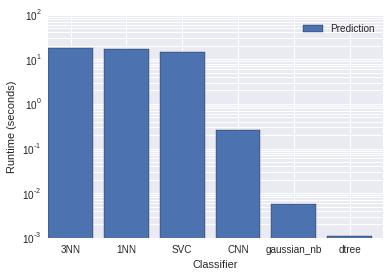
\includegraphics[scale=0.65]{figures/chapter_3/fig_3_13}
	\caption{不同算法分类时间}	\label{sec:fig_3_13}
\end{figure}
DTREE具有最低的分类时间,而KNN所需分类时间最多。
这主要是因为KNN在分类时,是将所有的训练样本进行比较,而且分类时间与样本数目多少成正相关,所以具有很高的分类时间;
决策树本身因为模型比较简单,只需要在树的少量分支上进行一定的运算,因此可以对数据进行快速分类。
SVM、DNN、CAE-CNN算法在进行分类时,需要进行一定的数据运算,因此分类时间也较长。
虽然CAE-CNN相较于其他算法在性能上没有明显的优势,但是考虑到小样本的分类本身启动GPU就耗费一定的时间,
而且其分类时间并没有很大,这也算一个可以接受的水平。
\par

\section{本章小结}

本章首先研究了通过无监督和有监督的方式所提取的数据特征之间的差异,
发现通过无监督的方法对数据样本进行特征提取可以重构原始数据样本,并获得原始样本具有一定类可分性的特征,
但是不同类别之间的数据会产生一定的混淆。
而通过有监督的方式获取的数据特征,对于不同调制方式而言,具有较强的类可分性,利用t-SNE算法将其映射到二维流型中,
发现同一类别的数据样本分布在低维流型中相近的区域,不同类别的样本分布在低维流型中的不同区域。
利用以上结论,我们提出了一种CAE-CNN调制识别的算法框架,并提出了一种相应的训练算法。
结果显示,我们提出的CAE-CNN算法,
在高信噪比条件下具有较高的识别准确率,并且鲁棒性较强;在低信噪比条件下也具备更高的识别率。
在算法效率上,我们提出的算法训练时间在可接受范围以内,同时算法运行时间较短,算法运行复杂度较低。\par

